\documentclass{article}

\usepackage{amsmath,amssymb,graphicx,geometry,enumitem}
\usepackage{xepersian}

\newcounter{qnumber}
\setcounter{qnumber}{1}

\newcommand{\Q}{
\textbf{سوال \theqnumber)}
\stepcounter{qnumber}
}

\setlength{\parindent}{0mm}
\setlength{\parskip}{3mm}
\settextfont{XB Niloofar}

\begin{document}

\begin{center}
\Large

به نام او

آزمون میان ترم سیگنال ها و سیستم ها
\end{center}

\hrulefill

\large

\Q
با بیان دلایل کافی، بررسی کنید هر یک از سیستم های پیوسته‌ی زیر، کدام ویژگی های علی بودن، خطی بودن، پایدار بودن، مستقل از زمان بودن و معکوس پذیری را دارا هستند (در هر یک از این سیستمها، $x(t)$ ورودی و $y(t)$ خروجی سیستم است).

الف) 
$
y(t)=x(t)x(t-2)
$

ب) 
$
y(t)=x(t)\delta(2t-1)
$

پ)
$
y(t)=\begin{cases}
e^{x(t)}&,\quad x(t)<0\\
\int_{-\infty}^t x(\tau+2)d\tau&,\quad x(t)\ge 0
\end{cases}
$

ت)
$
y(t)=\begin{cases}
x(-t)&,\quad t<0\\
x(t)&,\quad t\ge 0
\end{cases}
$

\Q

اگر سیگنال $x(t)$ به شکل زیر باشد و تبدیل فوریه آن را با 
$
X(j\omega)
$
نشان دهیم، بدون محاسبه مستقیم $X(j\omega)$ موارد زیر را بیابید.

الف)
$X(j0)$

ب)
$\int_{-\infty}^\infty X(j\omega) \frac{\sin \omega}{\omega} e^{j\omega}d\omega$

\begin{figure}[h]
\centering
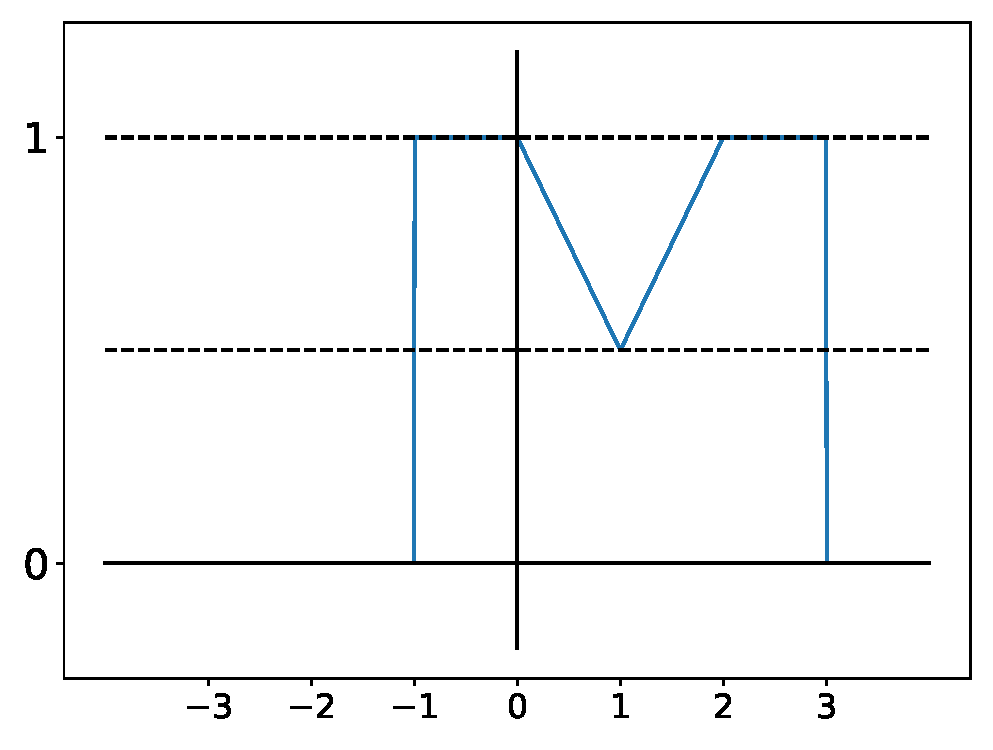
\includegraphics[width=80mm]{x13(t)}
\end{figure}

\Q

به یک سیستم LTI با تابع انتقال 
$$
H(j\omega)=\begin{cases}
\omega^2&,\quad |\omega|<4\\
0&,\quad \text{سایر جاها}
\end{cases}
،
$$
ورودی متناوب $x(t)$ مطابق شکل زیر داده می‌شود. خروجی این سیستم را بیابید.
\begin{figure}[h]
\centering
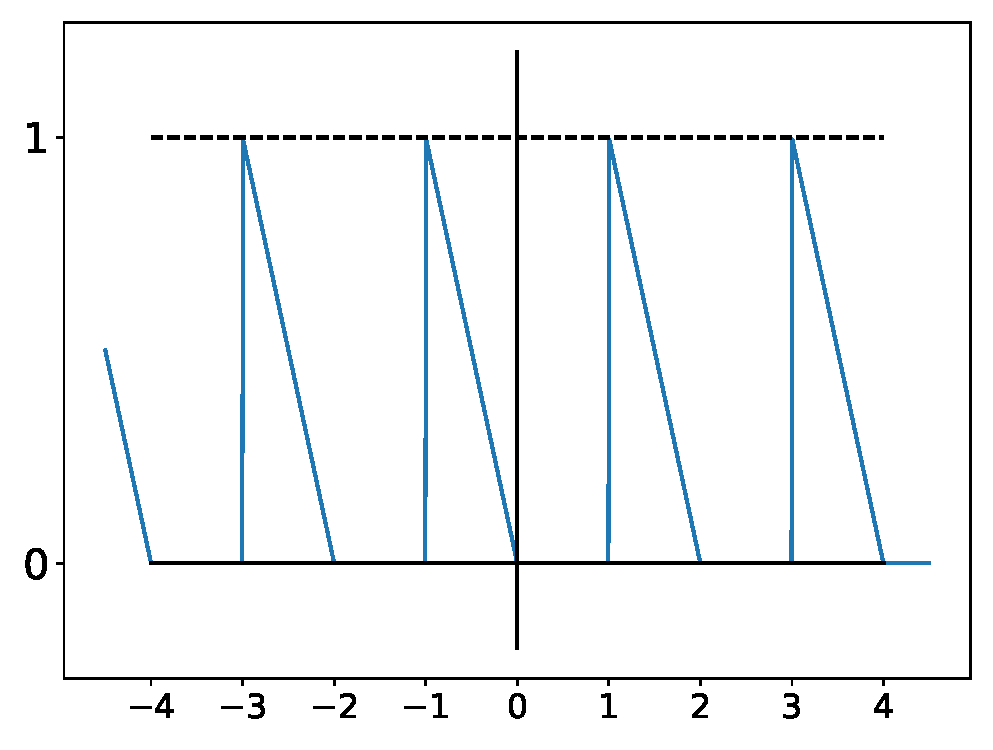
\includegraphics[width=75mm]{x3(t)}
\end{figure}

\Q
پاسخ یک سیستم LTI به ورودی 
$
x(t)=2e^{t}u(-t+1)
$
برابر 
$
y(t)
$
و پاسخ آن به ورودی 
$
\frac{dx(t)}{dt}
$
برابر 
$
y(t)-e^{-2|t|}
$
است. پاسخ ضربه این سیستم را بیابید.

\Q
اطلاعات زیر در مورد یک سیستم زمان-پیوسته‌ی LTI داده شده است:

\begin{enumerate}
\item
پاسخ ضربه سیستم، $h(t)$، حقیقی و زوج است.
\item
تبدیل لاپلاس سیستم دارای دو قطب و دو صفر بوده که یک صفر آن در $s=-2$ است.
\item
پاسخ این سیستم به ورودی 
$
x(t)=e^{jt}
$
برابر 
$
\frac{1}{2}e^{jt}
$
 است.
\item
$H(0)=1$
\end{enumerate}

پاسخ ضربه این سیستم را بیابید.

\Q
به سیستم غیر علی با تابع انتقال 
$
H(s)=\frac{2e^s}{s-3}
$،
ورودی 
$
x(t)=e^{-|t|}
$
داده می شود. در این صورت، خروجی این سیستم را در حوزه زمان بیابید ($\Re\{\cdot\}$ قسمت حقیقی عدد مختلط را نشان می دهد).
%\Q
%
%نمودار صفر-قطب تبدیل لاپلاس یک سیستم LTI و پیوسته به صورت زیر است:
%

\end{document}